\documentclass[../main.tex]{subfiles}

\begin{document}
    \section{Methodology}
    In this section, the methodology for observing and
    analyzing \gls{intrusion} attempts on the
    \gls{medicolbox} will be outlined.
    A description of the phenomenon of interest,
    data collection methods, sampling strategy,
    data collection procedures, ethical considerations,
    data analysis approach, validity and reliability measures,
    and limitations of the study will be provided.

    \subsection{Phenomenon of Interest}
    The phenomenon of interest in this study is
    \gls{intrusion} attempts on the \gls{medicolbox}.
    The various aspects of \gls{intrusion},
    including the methods employed by intruders,
    their motivations behind the attempts,
    and the potential consequences of successful \glspl{intrusion},
    will be investigated. By understanding these aspects,
    the project aims to enhance the
    security and protection of the
    \gls{medicolbox} and the medications it contains.

    \subsection{Data Collection Methods}
    To collect data on \gls{intrusion} attempts,
    the project will primarily utilize the
    Inertial Measurement Unit (\gls{imu}) as the
    main data collection method for detecting
    \gls{intrusion} attempts on the \gls{medicolbox}.
    This choice allows for a more focused investigation into the
    effectiveness of the \gls{imu} in identifying unauthorized access.

    The \gls{imu}, with its capability to capture physical movements,
    vibrations, and orientation changes of the \gls{medicolbox},
    provides valuable data for \gls{intrusion} detection and analysis.
    By relying on the \gls{imu} alone,
    the project aims to determine if it can effectively detect and
    alert on \gls{intrusion} attempts without the
    need for additional systems.

    This approach also enables the project to address the
    feasibility of implementing other
    data collection methods mentioned earlier,
    such as motion sensors, video surveillance,
    access logs, incident reports, and interviews.
    By evaluating the standalone performance of the \gls{imu},
    the project can assess its potential to serve as a cost-effective and
    efficient solution for \gls{intrusion} detection on the \gls{medicolbox}.

    The investigation will involve testing and analysis of the
    \gls{imu} data collected during simulated \gls{intrusion} attempts.
    This evaluation will focus on assessing the accuracy, reliability,
    and timeliness of the \gls{imu} in detecting and
    alerting on unauthorized movements or tampering.

    By dedicating the study to evaluating the \gls{imu}'s effectiveness as
    a standalone solution, the project aims to determine if the
    implementation of additional data collection methods is necessary for
    robust \gls{intrusion} detection.
    The results will provide insights into the suitability and viability of
    relying solely on the IMU for enhancing the security and
    protection of the \gls{medicolbox} and its contents.

    (Table \ref{tab:PotentialDataCollectionMethodsForIntrusionAttempts})
    presents potential data collection methods for \gls{intrusion} attempts.

    \begin{table}[htbp]
        \centering
        \caption{Potential Data Collection Methods for Intrusion Attempts}
        \label{tab:PotentialDataCollectionMethodsForIntrusionAttempts}
        \begin{tabular}{|l|p{10cm}|}
            \hline
            \textbf{Data Collection Method} & \textbf{Description} \\
            \hline
            Motion Sensors &
            Implementing motion sensors that can detect
            unauthorized movements near the \gls{medicolbox}. \\
            \hline
            Inertial Measurements (\gls{imu}) &
            Utilizing an Inertial Measurement Unit (\gls{imu}) to
            detect any changes in the orientation or
            movement of the \gls{medicolbox},
            providing data for \gls{intrusion} detection and analysis. \\
            \hline
            Video Surveillance &
            Installing surveillance cameras around the
            \gls{medicolbox} to capture \gls{intrusion} attempts visually. \\
            \hline
            Access Logs &
            Maintaining detailed logs of access attempts and
            recording any suspicious activities. \\
            \hline
            Incident Reports &
            Gathering information from incident reports filed by
            security personnel or individuals who
            have witnessed \gls{intrusion} attempts. \\
            \hline
            Interviews &
            Conducting interviews with security personnel to
            gain insights into their experiences and
            observations regarding \gls{intrusion} attempts. \\
            \hline
        \end{tabular}
    \end{table}

    The \gls{imu}, with its capability to capture physical movements,
    vibrations, and orientation changes of the \gls{medicolbox},
    provides valuable data for \gls{intrusion} detection and analysis.
    By relying on the \gls{imu} alone, the project aims to determine if
    it can effectively detect and alert on \gls{intrusion} attempts without the
    need for additional systems.

    This approach also enables the project to address the feasibility of
    implementing the other data collection methods mentioned earlier,
    such as motion sensors, video surveillance, access logs,
    incident reports, and interviews.
    By evaluating the standalone performance of the \gls{imu},
    the project can assess its potential to serve as a cost-effective and
    efficient solution for \gls{intrusion} detection on the \gls{medicolbox}.

    The investigation will involve comprehensive testing and analysis of the
    \gls{imu} data collected during simulated \gls{intrusion} attempts.
    This evaluation will focus on assessing the accuracy, reliability,
    and timeliness of the \gls{imu} in detecting and
    alerting on unauthorized movements or tampering.

    By dedicating the study to evaluating the
    \gls{imu}'s effectiveness as a standalone solution,
    the project aims to determine if the implementation of
    additional data collection methods is
    necessary for robust \gls{intrusion} detection.
    The results will provide insights into the suitability and
    viability of relying solely on the \gls{imu} for enhancing the
    security and protection of the \gls{medicolbox} and its contents.

    \clearpage

    \subsection{Prototype Construction}
    \begin{figure}[htbp]
        \centering
        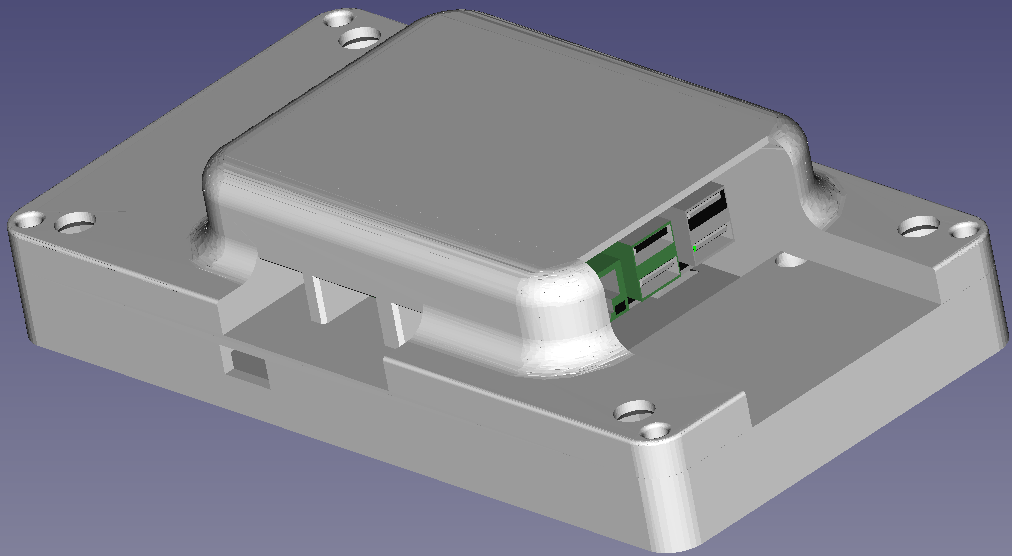
\includegraphics[width=0.7\textwidth]{resources/images/rpi_with_cover.png}
        \caption{Design of the prototype with the cover on}
        \label{fig:prototype_graphics_with_cover}
    \end{figure}

    The prototype control system is constructed using the following components:

    \begin{itemize}
        \item 1$\times$ Single-board computer: Raspberry Pi 4B 8 GB [9] as the CCU
        \item 1$\times$ Human-Machine Interface (HMI): 7-inch touchscreen [10]
        \item 1$\times$ Sensor Card: Raspberry Pi Sense Hat v1.0.0 [11] with an integrated IMU
        \item 4$\times$ M3 8 mm long threaded screws
        \item 8$\times$ M3 8 mm long spacers with 8 mm threaded rods on one side
        \item 1$\times$ 22-pin 0.5 mm pitch cable for the \gls{dsi} connectors
        \item 1$\times$ \gls{usb} type A to \gls{usb} type micro B cable for power and GND between HMI and Raspberry Pi
        \item 1$\times$ \gls{usb} type A to \gls{usb} type C cable for power
        \item 1$\times$ 230 V AC to \gls{usb} type A power adapter
        \item 1$\times$ Custom-designed cover to protect the electronics during testing
        \item 4$\times$ M3.5 8 mm long screws
        \item 4$\times$ M4 10 mm long screws
    \end{itemize}

    \begin{figure}[htbp!]
        \centering
        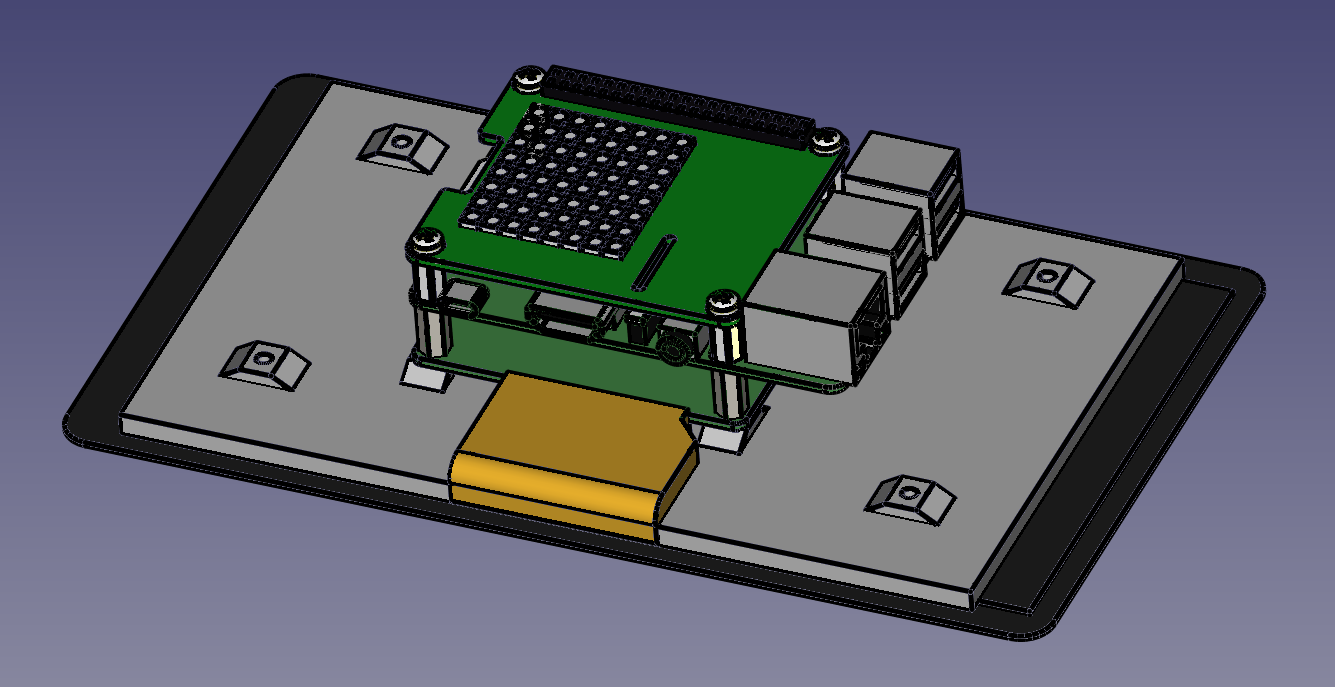
\includegraphics[width=0.7\textwidth]{resources/images/rpi_without_cover.png}
        \caption{Design of the prototype without the cover}
        \label{fig:prototype_graphics_without_cover}
    \end{figure}

    \clearpage

    The construction process involves the following steps:

    \begin{enumerate}
        \item Assemble the prototype:
        \begin{enumerate}
            \item Mount the Raspberry Pi 4B on the 7-inch touchscreen by using the threaded spacers.
            \item Mount the Raspberry Pi Sense Hat on the Raspberry Pi 4B by attaching it to the 2$\times$20 pin.
        \end{enumerate}
        
        \item Connect the components according to the wiring diagram (Figure \ref{fig:wiring_diagram}):
        \begin{enumerate}
            \item Connect the \gls{dsi} output from the Raspberry Pi to the \gls{dsi} input on the 7-inch touchscreen using a suitable ribbon cable.
            \item Connect the display's USB type micro B power connector input to one of the USB type A connectors on the Raspberry Pi (it does not matter which one).
        \end{enumerate}

        \item Enclose the electronics with the custom-designed cover.
        \begin{enumerate}
            \item Attach the screen to the first part of the casing using the M3.5 screws.
            \item{Attach the second part of the casing to the first part of the casing using the M4 screws.}
        \end{enumerate}
        
        \item Configure the software environment for the Raspberry Pi 4B and install the necessary libraries and drivers.
        \begin{enumerate}
            \item Open Raspberry Pi Imager. Install it if you don't already have.
            
            \item Insert the micro SD card into you computer. You can use adapter if needed.
            
            \item On Raspberry Pi Imager, select the storage device to install the operating system. Select the micro SD card.
            
            \item On Raspberry Pi Imager, select operating system to install. Select Raspberry Pi OS.
            
            \item Click \enquote{write} and wait til complete.
            
            \item Remove the micro SD card and insert it into the Raspberry Pi.
            
            \item start the Raspberry Pi, open terminal and type the code:
            \begin{verbatim}
                sudo raspi-config
            \end{verbatim}
            
            \item Select “Interfacing Options”
            
            \item Select the “I2C” option
            
            \item Select “<Yes>”

            \item Select “<Ok>”
            
            \item Select “<Yes>”
        \end{enumerate}

        \item Establish communication between the CCU, HMI, and the sensor card by setting up appropriate interfaces and protocols.
        \begin{enumerate}
            \item implement software that follows this sequence (Figure \ref{fig:sequence_diagram})
        \end{enumerate}
        
    \end{enumerate}

    \begin{figure}[htbp]
        \centering
        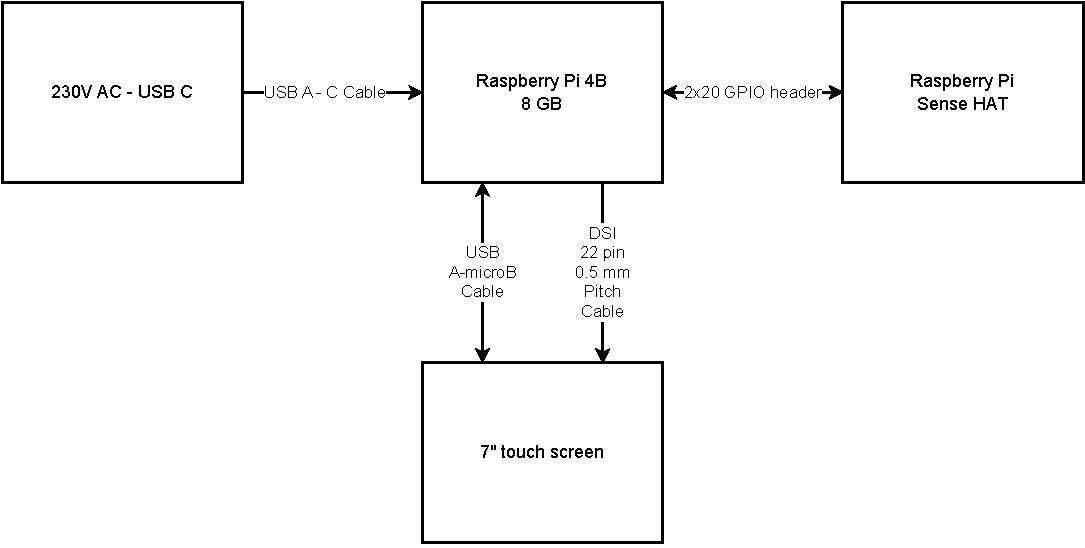
\includegraphics[width=0.8\textwidth]{resources/figures/Wiring.drawio.pdf}
        \caption{The \enquote{wiring diagram} used}
        \label{fig:wiring_diagram}
    \end{figure}
    
    \begin{figure}[htbp]
        \centering
        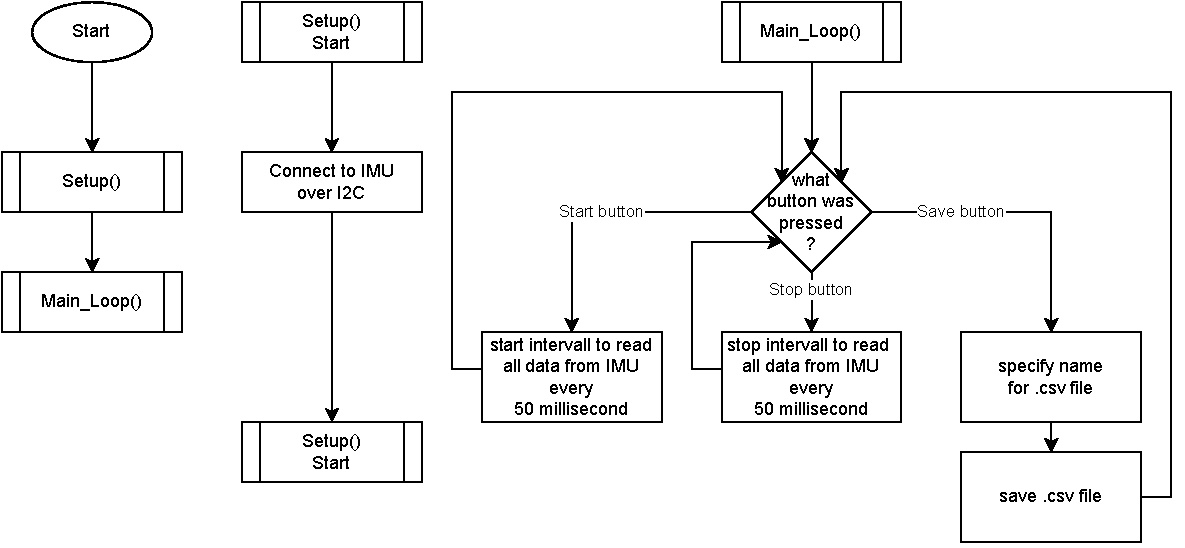
\includegraphics[width=0.8\textwidth]{resources/figures/sequence.drawio.pdf}
        \caption{The Sequence diagram used for the program}
        \label{fig:sequence_diagram}
    \end{figure}
    
    \begin{figure}[htbp]
        \centering
        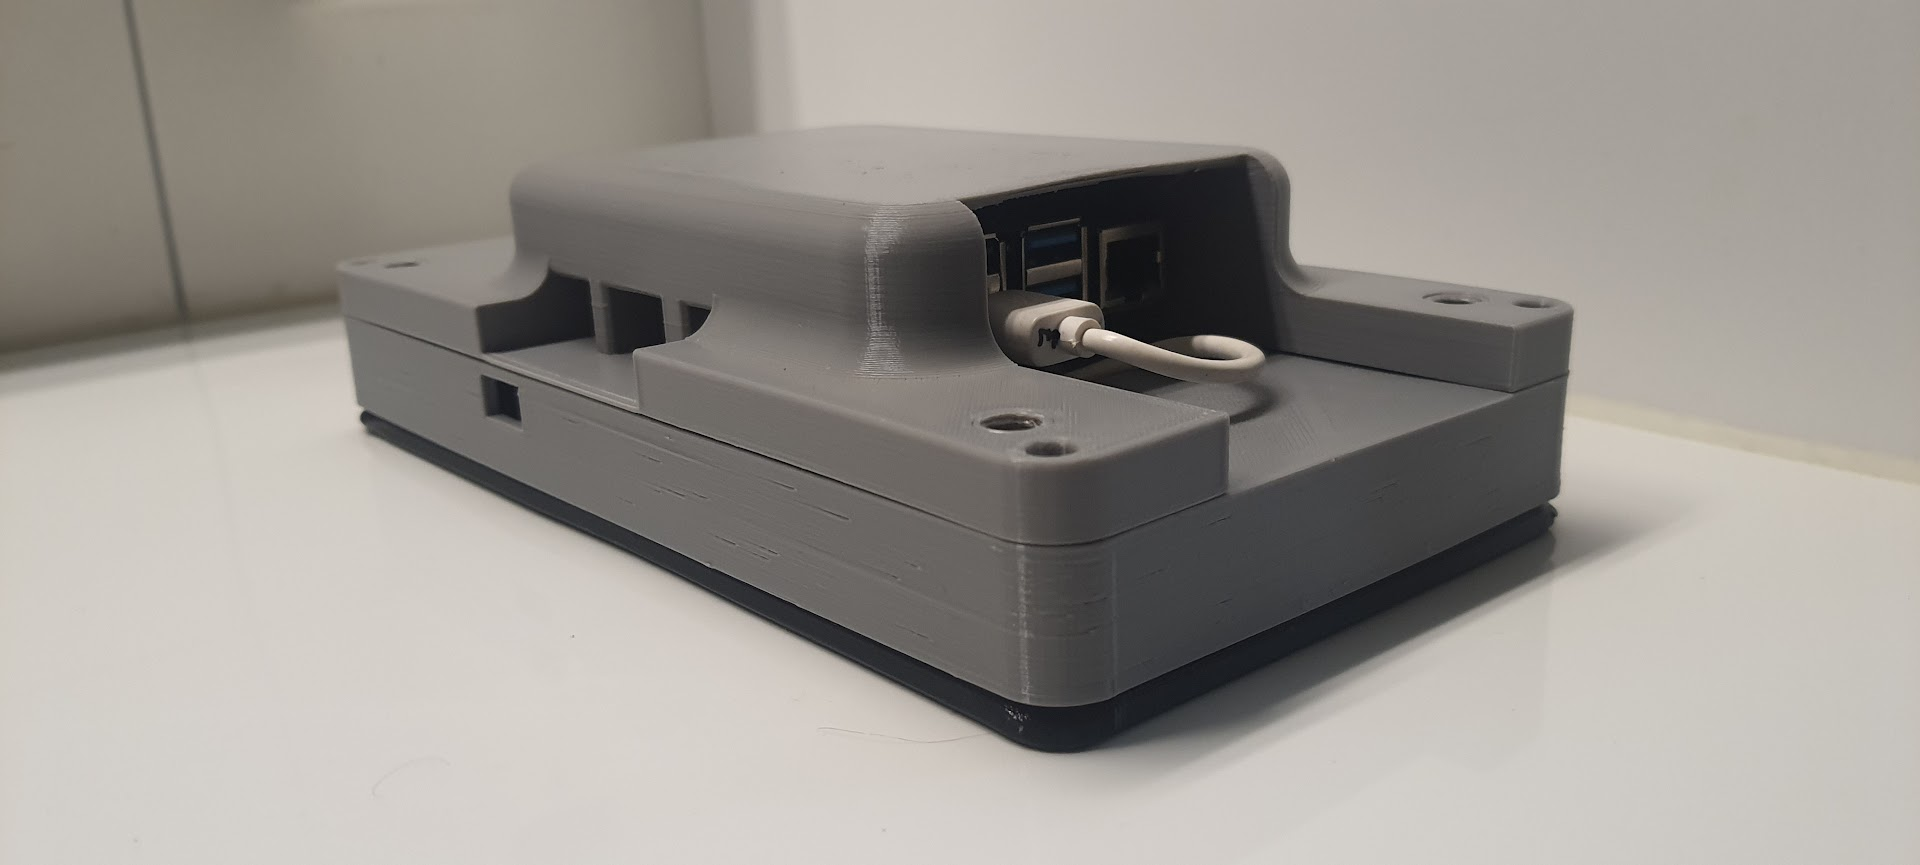
\includegraphics[width=0.8\textwidth]{resources/images/prototype_image.jpg}
        \caption{Photograph of the prototype}
        \label{fig:prototype_image}
    \end{figure}

    \subsection{Sampling Strategy}

    For our study, we define a sampling strategy to ensure the
    representation of different scenarios and potential risks associated with
    \gls{intrusion} attempts on the \gls{medicolbox}.
    Our sample may include specific locations where the \gls{medicolbox} is deployed,
    instances of reported \gls{intrusion} attempts,
    or a combination of both. We strive to select a diverse sample that covers a range of
    demographic and environmental factors to enhance the generalizability of our findings.

    \subsection{Data Collection Procedures}

    To collect data on \gls{intrusion} attempts, we follow specific procedures to
    ensure accuracy and completeness. These procedures involve implementing the
    following data collection methods (Table \ref{tab:DataCollectionMethods}):

    \begin{table}[htbp]
        \centering
        \caption{Possible Data Collection Methods for Intrusion Attempts}
        \label{tab:DataCollectionMethods}
        \begin{tabular}{|l|p{10cm}|} \hline
            \textbf{Data Collection Method} & \textbf{Description} \\ \hline
            Installing Surveillance Cameras and Motion Sensors &
            Installing surveillance cameras and motion sensors at strategic locations around the \gls{medicolbox}. \\ \hline
            
            Implementing Protocols for Incident Documentation &
            Implementing protocols for documenting and reporting \gls{intrusion} incidents, including recording timestamps, descriptions of the events, and any available contextual information. \\ \hline
            
            Reviewing Video Footage, Access Logs, and Incident Reports &
            Regularly reviewing video footage, access logs, incident reports, and conducting interviews to gather relevant data. \\ \hline
            
            Ensuring Equipment Functionality and Maintenance &
            Ensuring the proper functioning and maintenance of surveillance equipment and data storage systems. \\ \hline
        \end{tabular}
    \end{table}
    
    These procedures help us capture the necessary data for analysis and provide a
    comprehensive understanding of \gls{intrusion} attempts on the \gls{medicolbox}.

    \subsection{Ethical Considerations}

    We recognize and address ethical considerations related to our study. This includes:

    \begin{itemize}
        \item Adhering to relevant data protection regulations and guidelines.
        \item Anonymizing data during the analysis phase to protect the identities of individuals involved.
    \end{itemize}

    By considering these ethical considerations,
    we aim to conduct our study with integrity and respect for individuals' privacy.

    \subsection{Data Analysis}

    The collected data from the \gls{imu} is analyzed using a systematic approach.
    Since there is no video footage or access logs available,
    our analysis focuses solely on the data captured by the \gls{imu}.
    The analysis process includes the following steps:
    
    \begin{itemize}
    \item Data preprocessing: The collected \gls{imu} data is preprocessed to ensure its quality and suitability for analysis. This may involve removing any noise or outliers, normalizing the data, and performing any necessary transformations to prepare it for further analysis.
    \item Exploratory data analysis: We conduct exploratory data analysis to gain a better understanding of the \gls{imu} data. This involves visualizing the data, examining summary statistics, and identifying any patterns or trends that may be present. Exploratory analysis helps in identifying initial insights and forming hypotheses for further investigation.

    \item \gls{intrusion} detection algorithm: We develop or utilize an \gls{intrusion} detection algorithm that can process the \gls{imu} data and identify potential \gls{intrusion} attempts. This algorithm is trained and validated using a suitable methodology to ensure its effectiveness in detecting unauthorized access based on the \gls{imu} readings.

    \item Statistical analysis: If applicable, statistical analysis techniques can be employed to analyze the \gls{imu} data further. This may include identifying correlations between different variables or conducting hypothesis testing to validate any observed patterns or relationships.

    \item Data visualization: Data visualization techniques, such as plots, charts, or graphs, can be employed to present the analyzed \gls{imu} data effectively. Visualizations can help in understanding the patterns, trends, and anomalies in the data, making it easier to interpret and communicate the findings.
    
    \end{itemize}

    \clearpage

    By conducting an analysis of the anonymized \gls{imu} data,
    we aim to gain insights into the effectiveness of the
    \gls{imu} in detecting \gls{intrusion} attempts on the \gls{medicolbox}.
    This analysis will contribute to the assessment of the \gls{imu} as a
    standalone solution for enhancing the security and
    protection of the \gls{medicolbox} and its contents.

    \subsection{Limitations}        
    It is essential to acknowledge the limitations inherent in
    studying \gls{intrusion} attempts on the \gls{medicolbox}.
    These limitations may include:
        
    \begin{itemize}
        \item \textbf{Availability of \gls{intrusion} data:} The limited availability of documented \gls{intrusion} attempts may impact the sample size and the generalizability of the findings.

        \item \textbf{Challenges in capturing all \gls{intrusion} attempts:} Some \gls{intrusion} attempts may go undetected or unreported, leading to potential underrepresentation in the collected data.

        \item \textbf{Generalizability of findings:} The context of the \gls{medicolbox} and the specific locations where it is deployed may influence the generalizability of the findings to other similar systems.
    \end{itemize}
    
    We address these limitations by maximizing the available data,
    selecting a diverse sample, and providing contextual information to aid in the
    interpretation and application of our findings.
    
    By incorporating these elaborations into the methodology section,
    we can effectively observe and analyze \gls{intrusion} attempts on the
    \gls{medicolbox}, gaining insights into the methods,
    motivations, and potential vulnerabilities associated with these attempts.
    \subsection{Tools and Technologies}

During the course of this study, the following tools and technologies were utilized:

\begin{itemize}
    \item \textbf{LaTeX:} LaTeX, a typesetting system widely used in academia and scientific research, was used for document preparation. It provided powerful tools for creating professional-looking documents, including support for mathematical equations, figures, tables, and bibliographic references.
    
    \item \textbf{Visual Studio Code (VSCode):} VSCode, a versatile text editor, served as the primary tool for writing code, editing documents, and managing project files. It provided a user-friendly interface, syntax highlighting, code completion, and integration with version control systems like Git.
    
    \item \textbf{FreeCAD:} FreeCAD, an open-source computer-aided design (CAD) software, was utilized for designing and creating 3D models of the prototype. It enabled precise modeling and visualization of the physical components, ensuring accurate representation and construction.
    
    \item \textbf{GitHub:} GitHub, an open-source web-based platform for version control and collaboration, was used to track changes, collaborate with team members, and maintain the integrity and availability of project files. It provided a centralized repository for source code and project documentation.
    
    \item \textbf{Programming Languages:} The primary programming languages used in this study were Python and JavaScript. Python, an open-source language, was employed for data analysis, algorithm development, and system control, while JavaScript, also open-source, was utilized for web development and implementing the human-machine interface (HMI) functionality.
    
    \item \textbf{Electron:} Electron, an open-source framework for building cross-platform desktop applications, was utilized for developing the HMI. It enabled the integration of open-source web technologies (HTML, CSS, and JavaScript) into a standalone application, providing a responsive and user-friendly interface.
\end{itemize}

These open-source tools and technologies played a crucial role in streamlining the research process, facilitating data analysis, and developing a functional prototype that aligns with the research objectives. By prioritizing open-source solutions, the study fostered collaboration, transparency, and accessibility, promoting the advancement of knowledge and encouraging community contributions.

\subsection{Document Preparation}

The document was prepared using LaTeX, an open-source typesetting system widely used in academia and scientific research. LaTeX provided powerful tools for creating professional-looking documents, including support for mathematical equations, figures, tables, and bibliographic references.

To facilitate the writing process, Visual Studio Code (VSCode), an open-source text editor, was utilized as the primary tool. VSCode offered a range of features and extensions that enhanced productivity and provided a seamless writing experience. It enabled efficient collaboration, syntax highlighting, code completion, and integration with version control, ensuring the integrity and consistency of the document.

By leveraging open-source tools like LaTeX and VSCode, the study embraced the principles of openness, collaboration, and knowledge sharing, fostering innovation and contributing to the open-source community.

\end{document}
